\chapter{Conclusion}\label{ch:conclusion}
Driving the performance limits of optical microscopy systems requires a unique blend of both hardware and software innovations. Among a wide variety of techniques for probing a sample, coded illumination using a programmable light source is advantageous due to its simplicity and wide utility for various computational imaging techniques. In this work, we proposed a variety of techniques which take advantage of programmable illumination to enable label-free contrast, quantitative imaging, and high-throughput imaging at relatively low cost and complexity on existing optical systems. We have leveraged novel hardware and computational techniques to push performance boundaries in critical areas, such as label-free imaging and neuropathology. Further, we have put significant effort towards quantifying when computational techniques do not provide benefit, acknowledging limiting cases where conventional methods are still state-of-the-art. Taken together, the methods presented in this work illustrate the capabilities of a computational imaging system, and offer evidence of the impact these systems could have on the broader microscopy community.

\begin{wrapfigure}{R}{15em}
  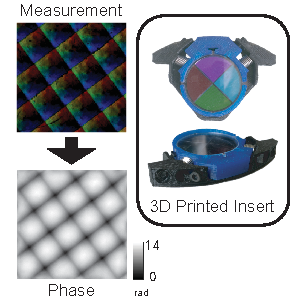
\includegraphics[width=\linewidth]{avatar_phase}
\end{wrapfigure}

In Chapter~\ref{ch:phase} we described differential phase contrast (DPC), a quantitative phase imaging method which uses partially coherent illumination to recover the complex field of a thin (weak) object. We then introduced a single-shot variant of DPC which uses  color-multiplexed illumination to recover the linearized optical field from a single measurement. Our hardware requirements are simple, inexpensive, and compatible with most commercial microscopes through of the use of a color camera and a simple color filter insert placed at the back focal plane of the condenser lens, the same position as many removable phase contrast annulus rings. Unlike phase contrast and DIC, our method does not require special objectives or prisms, which reduces our hardware costs to that of the 3D printed filter itself. In addition, we can use our quantitative phase and amplitude methods to synthesize phase contrast and DIC images digitally, matching the functionality of existing phase imaging systems at a fraction of the cost. Finally, we presented a framework for analyzing the source design for DPC-based system in terms of SNR and explored source calibration and measurement count as examples of this analysis.

\begin{wrapfigure}{L}{15em}
  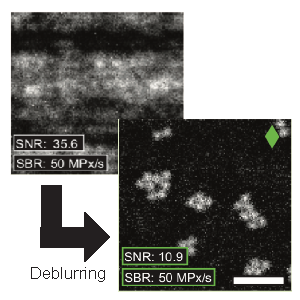
\includegraphics[width=\linewidth]{avatar_highthroughput}
\end{wrapfigure}

In Chapter~\ref{ch:highthroughput}, we introduced the concept of high-throughput imaging, and described conventional methods for obtaining images with a wide field-of-view and high resolution. After discussing the limitations of existing methods, we proposed a novel coded illumination technique where measurements are acquired while the sample is in motion, which is synchronized with multiple illumination pulses during each exposure to introduce a known motion blur. These images, which have higher SNR than images captured at the same speed under strobed illumination, are then computationally deblurred to recover the static object at high speed while maintaining the SNR of much slower acquisition methods. We compare our technique to existing methods, stop-and-stare and strobed illumination, which require a significantly longer acquisition time or produce images with significantly lower SNR, respectively. Using a generalized framework for predicting the reconstruction SNR of measurements acquired using each method, we show, through both theory and experiment, that our coded illumination technique can produce images with up to 10$\times$ the SNR of strobed acquisitions, at significantly faster acquisition rates than images captured under strobed illumination.

\begin{wrapfigure}{R}{12em}
  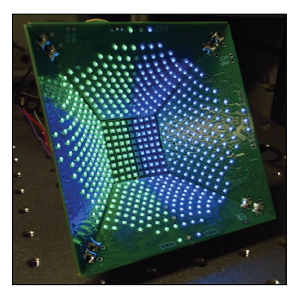
\includegraphics[width=\linewidth]{avatar_fabrication}
\end{wrapfigure}

\noindent of this benefit is not constant across system parameters such as camera readout noise and illumination power. To quantify how our method compares to existing methods, we perform an analysis of the relative performance of our method compared to conventional high-throughput imaging techniques such as strobed illumination or stop-and-stare. For low-light situations such as fluorescence imaging, our method is uniquely suited to provide faster imaging at higher SNR than existing methods.


In Chapter~\ref{ch:fabrication}, we detail the design and fabrication of coded illumination devices for the computational microscopy applications presented in this dissertation. We begin by defining the common design requirements of programmable illumination devices, focusing on programmable LED arrays as our primary application due to their low cost and wide availability. We then describe several design iterations of a programmable LED dome which enables high-angle coded illumination. In the first design iteration, we designed and fabricated a 3D-printed LED dome which was carefully assembled by hand, requiring several months of fabrication. This device was intended to be used with CellScope, a portable microscope platform which uses a smartphone to capture and process images for telemedicine applications. In the second design iteration, we designed and developed a LED quasi-dome which uses 5 printed-circuit boards arranged in a dome-like structure. This device requires significantly less time and effort to assemble and provides RGB illumination across 581 LEDs up to 0.9NA. The ease of manufacturing has enabled the wide distribution of these devices to collaborators around the world. Finally, we describe the Computational CellScope platform in greater detail, which implements coded illumination on a portable platform to perform digital refocusing using light-field methods, quantitative phase imaging, and multi-contrast imaging.


\begin{wrapfigure}{L}{15em}
  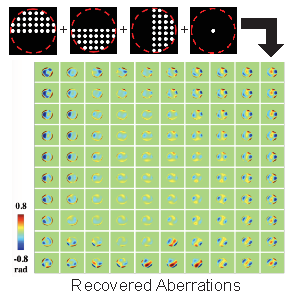
\includegraphics[width=\linewidth]{avatar_selfcal}
\end{wrapfigure}


In Chapter ~\ref{ch:selfcal}, two methods for self-calibration of computational imaging systems are described. Computational imaging methods are uniquely susceptible to mis-calibration since the inferred forward model is often assumed to be ideally calibrated. In reality, the forward model is a function of the optical physics and optical design (which can be inferred), as well as mis-calibration, which cannot be assumed to be negligible in many systems. We first discuss a technique for performing aberration self-calibration using differential phase contrast. Our method employs an alternating-minimization approach to solve for both the complex field of the object as well as the aberrations, which are projected into a Zernike basis. This method is non-convex, but is differentiable, and guaranteed not to diverge so long as an appropriate step size is used. Further, we use a patch-wise solver to solve for aberrations across the field, revealing spatially variant aberration functions. We verify our method by solving for the defocus aberration when introducing a known defocus term. Our method requires only a single coherent measurement, in addition to three DPC measurements for recovering the object's complex field. Next, we presented a method for performing self-calibration of LED positions in both the brightfield and darkfield regions for Fourier ptychography. After performing a brightfield calibration method, we employ a novel gradient-based technique for solving for the homography between printed circuit boards in a quasi-dome device. This technique makes the alternating minimization process much more stable and enables high-NA Fourier ptychography with resolution below 450nm. While a good hardware system alignment is most effective, these self-calibration techniques can mitigate mis-calibration when this is not possible.
\clearpage
\section{Proposed Future Work}
As my time at Berkeley comes to a close, there are still many open questions which I find interesting and would like to pursue, given the opportunity. In the future, I hope that myself or someone else will have the time and a motivation to explore a few of the following proposals.

The first, and most general, is the application of a task-based imaging paradigm to the applications discussed in this work. In each of the previous chapters, we have quantified the quality of our reconstructions using system parameters such as signal-to-noise ratio, acquisition throughput (space-bandwidth rate), resolving power and field of view. Rarely is emphasis placed on the quality of these images towards a specific task, such as cell counting, pathogen recognition, or disease diagnosis. Conventionally the field of computational imaging has tended to focus on imaging system performance, but I believe that defining a differentiable performance metric (cost function) which is relevant to the imaging task would be extremely interesting. As a first step, I would propose cell-counting as a metric. Recent work from the machine learning community has proposed optimizing network layers for the counting and classification of cells~\cite{falk2019unet, xue2017cell}. Including programmable hardware elements (such as LED arrays which could introduce different contrast) into the learning pipeline could provide significant improvements in counting accuracy and performance.

A second, more specific future direction, is the application of compressed sensing to solve under-determined motion deblurring problems for slide-scanning and digital pathology applications. Currently, the volume of data required for large-scale imaging (e.g. neuropathology) can make acquisition times and data storage difficult or infeasible. If data acquisition processing requirements were lower, acquisitions could be made much faster, and large-scale imaging analysis could be more readily performed. For a compressed-sensing acquisition to perform well, the aliasing introduced by undersampling should be incoherent with a domain in which the sample is sparse. An acquisition with a random forward operator is one example of such a forward model, because this matrix is incoherent with every other matrix. While it is very difficult to design a truly random forward operator in this problem, we have control over the structure of our forward operator through the illumination sequence as well as the motion pathway. So long as this acquisition introduces incoherent aliasing, we have some hope of reconstructing a sparse object from an under-determined system. To accomplish this, I would propose optimizing the entire pipeline using an unrolled network, which allows us to differentiate with simple parameters such as step size as well as more complicated parameters, such as the sparsifying operator or acquisition strategy. Using large amounts of training data, we could then generate a principled acquisition and reconstruction strategy together which would enhance the capabilities of high-throughput acquisitions well-beyond those presented in this work.

A third future direction is active imaging, or the active determination of acquisition trajectories based on current image data. These trajectories need not span Cartesian space, but could also include LED angle, defocused positions, or other metrics. A key component to these methods being advantageous would be that the sample should be localized, meaning that most of the densely sampled data is unnecessary, and that the learning process should be fast, so that the compute + scan time does not exceed the time to densely scan a sample. An obvious example of this would be multi-well plates, where a microscope may perform a fast scan over many wells which aliases them together, then uses this blurred data to determine which wells are worth imaging more closely at high-resolution for quantification. Such a technique could speed up acquisitions significantly for many applications.

In terms of fabrication of LED devices, I believe that engineering improvements in the power supply of the devices as well as a more careful layout of the high-speed traces (such as serial clock and pulse-width-modulation clock) would enable imaging with shorter exposure times. In addition, a more compact portable microscope device incorporating a PCB-based LED array would be much more robust than the current Computational CellScope device, enabling wider distribution to collaborators around the world.

I have made much of my existing code available under the BSD open-source license at repositories listed in Appendix, Section~\ref{sec:appendix:opensource}. I hope that these examples and this dissertation will inspire others to iterate and advance the field of computational imaging.
